\documentclass{beamer}
\usepackage{amsmath}
\usepackage{graphicx}
\usepackage{subcaption}
\usepackage{todonotes}
\usepackage{physics}
\usepackage{booktabs}
\usepackage[
    backend=biber,
    natbib,
    style=nature
]{biblatex}
\usepackage{xcolor} % Required for custom colors
\usepackage{hyperref}
\usepackage{multirow}
\addbibresource{examples.bib}

% Define custom colors
\definecolor{caltechorange}{RGB}{255,88,0}
\definecolor{caltechgray}{RGB}{102,102,102}

% Set Beamer colors
\setbeamercolor{title}{fg=caltechorange}
\setbeamercolor{frametitle}{fg=caltechorange}
\setbeamercolor{structure}{fg=caltechgray}
\setbeamercolor{itemize item}{fg=caltechorange}
\setbeamercolor{itemize subitem}{fg=caltechgray}
\setbeamercolor{block title}{fg=white,bg=caltechorange}
\setbeamercolor{block body}{bg=caltechgray!20}

% Custom command for colored boxes around equations
\newcommand{\highlight}[1]{\colorbox{caltechgray!10}{$\displaystyle#1$}}
\newcommand{\highlightorange}[1]{\colorbox{caltechorange!10}{$\displaystyle#1$}}


\title{\textcolor{caltechorange}{$G_0W_0$ for molecules}}
\institute{Caltech}
\author{\textcolor{caltechgray}{Patryk Kozlowski}}
\date{\today}

\begin{document}

\begin{frame}
    \titlepage
\end{frame}
\begin{frame}
    \frametitle{\textcolor{caltechorange}{Motivation}}
\textbf{Objective}: solve time-independent Schrödinger equation for $N$ electron system in the Born-Oppenheimer approximation
\begin{equation}
\highlight{\hat{H}\Psi_0 = E_0\Psi_0}
\end{equation}
\pause
where

\begin{equation}
\highlight{\hat{H} = \sum_{i=1}^N\left(-\frac{1}{2} \nabla_i^2\right) - \sum_{i=1}^N \sum_{\alpha}\frac{Z_{\alpha}}{r_{i\alpha}} + \sum_{i<j}^N \frac{1}{r_{ij}} + C_{nn}}
\end{equation}

\end{frame}

\begin{frame}
    \frametitle{\textcolor{caltechorange}{Common electronic structure tools}}
\begin{itemize}
    \item Mean-field theories
    \begin{itemize}
        \item \textbf{Hartree-Fock}: Assumes only average electron-electron interactions
        \item \textbf{Density Functional Theory}: Lack of systematic improvability due to the approximate exchange-correlation functional
    \end{itemize}
\pause
    \item Wavefunction-based methods
    \begin{itemize}
        \item \textbf{Coupled cluster theories like CCSD(T)}: Highly accurate, but computationally intractable for large systems
        \end{itemize}
\pause
    \item Green function methods
    \begin{itemize}
        \item \textbf{GW approximation}: The gap-filling method; decent accuracy for cheap computational cost
        \item variation of this ($G_0W_0$) studied here
    \end{itemize}
\end{itemize}
\end{frame}



\begin{frame}
    \frametitle{\textcolor{caltechorange}{Self-Energy}}
    \begin{figure}
        \caption{Electron gas propagation\autocite{mattuck_guide_1992}}
        \begin{subfigure}{.4\textwidth}
            \centering
            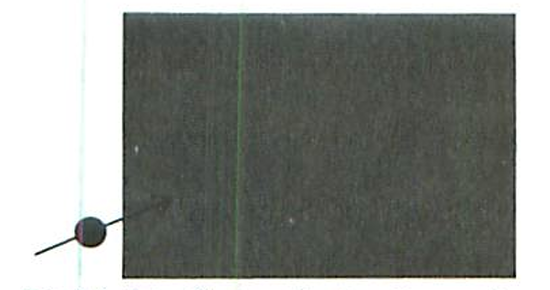
\includegraphics[width=.8\linewidth]{shot.png}
            \caption{The \textbf{bare} electron is shot into the gas}
            \label{fig:shot}
        \end{subfigure}
        \begin{subfigure}{.4\textwidth}
            \centering
            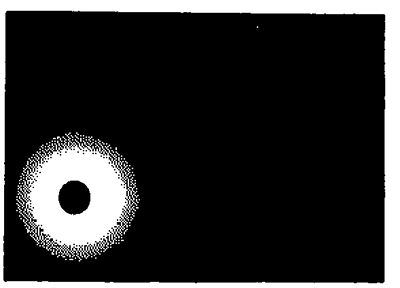
\includegraphics[width=.8\linewidth]{clothing.png}
            \caption{The \textbf{quasi}-electron dynamically creates holes}
            \label{fig:clothing}
        \end{subfigure}
        \label{fig:propagates}
    \end{figure}
\pause
    Qualitatively 
    \begin{equation}
        \highlight{\epsilon_{\text{self}} = \epsilon_{\text{quasi}} - \epsilon_{\text{bare}},}
    \end{equation}
    The \textbf{self-energy} $\Sigma $ can be thought of as the difference between the quasi and bare electron
\end{frame}



\begin{frame}
    \frametitle{\textcolor{caltechorange}{$G_0W_0$ iterative procedure \autocite{bruneval_assessment_2019} for $\varepsilon_{p}^{\mathrm{QP}}$}}
    \begin{equation}
\highlight{\epsilon_p^{\mathrm{MF}} + \Sigma_p^{\mathrm{corr}}(\varepsilon_p^{\mathrm{QP}}) = \varepsilon_p^{\mathrm{QP}}}
    \end{equation}
    \begin{enumerate}
        \item start with the mean-field guess $\epsilon_p^{\mathrm{MF}}$
        \item add self-energy, evaluated at $\varepsilon_p^{\mathrm{QP}}$ from the previous iteration
        \item iterate until self-consistency in $\varepsilon_p^{\mathrm{QP}}$ is reached
    \end{enumerate}
\pause
    \begin{table}[h]
    \centering
    \caption{Deviation in $\varepsilon_p^{\mathrm{QP}}$ (in eV) for $G_0W_0$ between my implementation and PySCF\autocite{sun_recent_2020}}
    \begin{tabular}{|c|c|c|c|c|}
    \hline
    \multirow{1}{*}{Orbital} & \multicolumn{1}{c|}{$H_2O$} & \multicolumn{1}{c|}{$NH_3$} & \multicolumn{1}{c|}{$LiH$} & \multicolumn{1}{c|}{$CO$} \\
    \hline
    HOMO - 2 & 5.33e-15 & 1.42e-14 & 3.55e-14 & 0.00477 \\
    \hline
    HOMO - 1 & 1.07e-13 & 2.33e-10 & 2.84e-14 & 0.00476 \\
    \hline
    HOMO     & 2.84e-13 & 1.30e-12 & 1.96e-10 & 2.84e-13 \\
    \hline
    LUMO     & 2.65e-14 & 8.78e-14 & 2.66e-15 & 0.00679 \\
    \hline
    LUMO + 1 & 2.71e-14 & 8.78e-14 & 2.43e-14 & 0.00678 \\
    \hline
    LUMO + 2 & 6.92e-10 & 4.97e-14 & 3.09e-14 & 3.99e-14 \\
    \hline
    \end{tabular}
    \end{table}
\end{frame}
\begin{frame}
    \frametitle{\textcolor{caltechorange}{Linearized $G_0W_0$ density matrix\autocite{bruneval_improved_2021}: Part 1}}
\textbf{Natural occupations}:  number of electrons in a given orbital.\autocite{szabo_modern_2012}
\begin{figure}[h]
    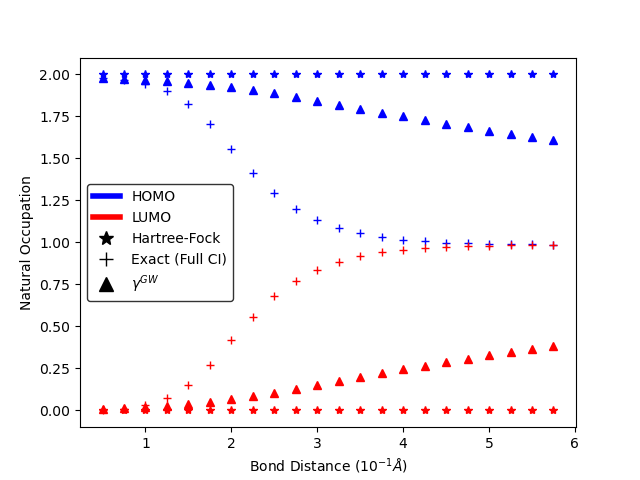
\includegraphics[width=0.9\textwidth]{h2_occupations.png}
\caption{HOMO and LUMO of $\mathrm{H_2}$ along the dissociation coordinate}

\end{figure}
\end{frame}
\begin{frame}
\frametitle{\textcolor{caltechorange}{Reference}}
    \begin{figure}[h]
    \centering
    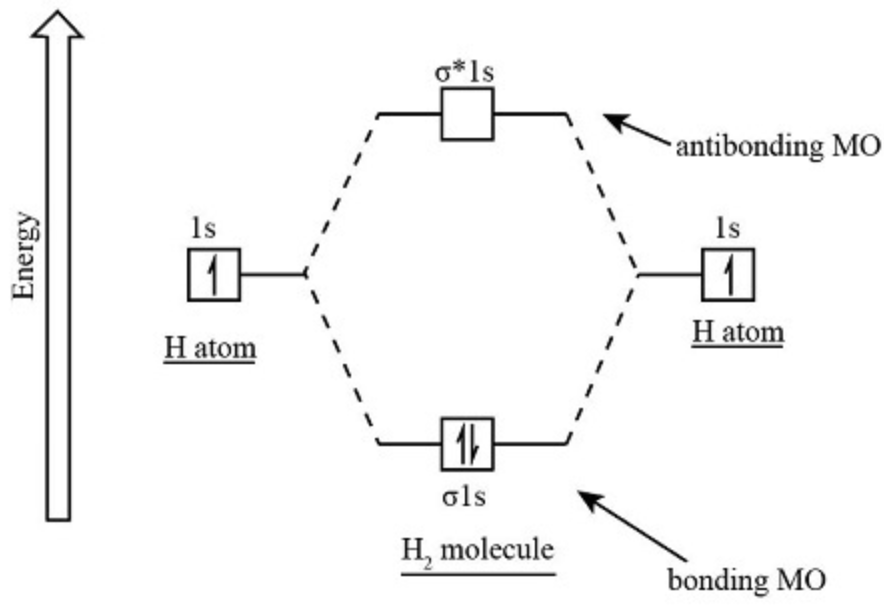
\includegraphics[width=\textwidth]{h2_mo.png}
\caption{MO diagram of $\mathrm{H_2}$ at the equilibrium bond distance \autocite{noauthor_molecular_nodate}}
\label{fig:h2_mo_diagram}
\end{figure}
\end{frame}

\begin{frame}
    \frametitle{\textcolor{caltechorange}{Total energies from the linearized $G_0W_0$ density matrix}}
{Galitskii-Migdal $E^{\mathrm{corr}}$}: convolution of the correlation self-energy $\Sigma _c$ with the Green's function $\mathcal{D}$
\begin{equation}
    \highlight{E_{\mathrm{corr}}^{\mathrm{GM}}=-\frac{\mathrm{i}}{2} \int_{-\infty}^{\infty} \frac{\mathrm{d} \omega}{2 \pi} \int \mathrm{d} \boldsymbol{x}_1 \boldsymbol{x}_3 e^{\mathrm{i} \omega \eta} \Sigma_{\mathrm{c}}\left(\boldsymbol{x}_1 \boldsymbol{x}_3 ; \omega\right) \mathcal{D}\left(\boldsymbol{x}_3 \boldsymbol{x}_1 ; \omega\right)}
\label{eq:GM_total_energy}
\end{equation}
\begin{table}[h!]
    \centering
    \caption{Deviation in total energies (in eV) {from the CCSD(T) reference} for Hartree-Fock and $\gamma ^{\mathrm{GW}}$ of the linearized $G_0W_0$ density matrix (using $E^{\mathrm{corr}}$ from equation \ref{eq:GM_total_energy}).}
    \begin{tabular}{|l|c|c|}
        \hline
        \textbf{Molecule} & \textbf{HF $\Delta $CCSD(T)} & \textbf{$\gamma ^{\mathrm{GW}}$ $\Delta $CCSD(T)} \\
        \hline
        \textbf{H$_2$O} & 5.93 & 0.696 \\
        \hline
        \textbf{NH$_3$} & 5.60 & 0.544 \\
        \hline
        \textbf{LiH} & 0.846 & 0.0361 \\
        \hline
    \end{tabular}
    \label{tab:total_energy_gm_ev}
    \vspace{-10pt}
\end{table}



\end{frame}
\begin{frame}
    \frametitle{\textcolor{caltechorange}{Acknowledgements}}
    I would like to thank the medical professionals who are the reason that I can be here, the guys at Cursorless who helped me learn to voice code, my adviser, Professor Garnet Chan, and mentor, Dr. Johannes Tolle, for guiding me in my research, and my family, and particularly my mom, for being the biggest supporters in my rehabilitation and academic journey.
\end{frame}





\begin{frame}
    \frametitle{\textcolor{caltechorange}{Bibliography}}
    \printbibliography
\end{frame}

\end{document}
